% -----------------------------------------------
% Template for ISMIR 2014
% (based on earlier ISMIR templates)
% -----------------------------------------------

\documentclass{article}

\usepackage{ismir2014,amsmath,cite,url,graphicx}
\usepackage[utf8]{inputenc}

\title{Spotify-ed: Music Recommendation and Discovery in Spotify}

% Single address
% To use with only one author or several with the same address
% ---------------
%\oneauthor
% {José Bateira}
% {Affiliations should be omitted for double-blind reviewing}

% Two addresses
% --------------
%\twoauthors
%  {José Bateira} {School \\ Department}
%  {Second author} {Company \\ Address}

% Three addresses
% --------------
\threeauthors
  {José Bateira} {Porto, Portugal \\ {\tt ei10133@fe.up.pt}}
  {Second author} {\bf Retain these fake authors in\\\bf submission to preserve the formatting}
  {Third author} {Affiliation3 \\ {\tt author3@ismir.edu}}

% Four addresses
% --------------
%\fourauthors
%  {José Bateira} {Affiliation1 \\ {\tt author1@ismir.edu}}
%  {Second author}{Affiliation2 \\ {\tt author2@ismir.edu}}
%  {Third author} {Affiliation3 \\ {\tt author3@ismir.edu}}
%  {Fourth author} {Affiliation4 \\ {\tt author4@ismir.edu}}

\begin{document}
%
\maketitle
%
\begin{abstract}
  There is an uncountable number of music streaming services that let the users play music, save their collection, create playlists and much more.
  Some services focus on creation and/or generation of playlists (8tracks \cite{8tracks}), others try to expand their music catalogue even further (Spotify \cite{spotify}, Rdio \cite{rdio}), while others focus more on personalized music recommendations (Pandora \cite{pandora}).

  Spotify presents music recommendations to the user with a list or a grid of suggestions, for example.
  However, lists do not provide the user enough information about the relation between the results \cite{Lamere2008}.
  A possible solution to this problem is to graphically represent the artist's similarities as a network of interconnected artists in a graph, where a node is a music artist, and each edge between them represents a connection.
  This is the concept that RAMA (Relational Artist MAps)\footnote{RAMA: \url{http://rama.inescporto.pt}}, a project developed at INESC Porto, uses \cite{Costa2008} \cite{Sarmento2009} \cite{Costa2009} \cite{Gouyon2011}.
  Spotify provides a way to build applications (plugin-like) that run \emph{inside} Spotify's Desktop Client \cite{spotifyapps}.
  A Spotify App is proposed in order to improve Spotify's presentation of recommendations by means of visual tools.

\end{abstract}
%
\section{Introduction}\label{sec:introduction}

  % 

\section{Page Size}\label{sec:page_size}

The proceedings will be printed on \underline{portrait A4-size paper} \underline{(21.0cm x 29.7cm)}.
All material on each page should fit within a rectangle of 17.2cm x 25.2cm,
centered on the page, beginning 2.0cm
from the top of the page and ending with 2.5cm from the bottom.
The left and right margins should be 1.9cm.
The text should be in two 8.2cm columns with a 0.8cm gutter.
All text must be in a two-column format.
Text must be fully justified.

\section{Typeset Text}\label{sec:typeset_text}

\subsection{Normal or Body Text}\label{subsec:body}

Please use a 10pt (point) Times font. Sans-serif or non-proportional fonts
can be used only for special purposes, such as distinguishing source code text.

The first paragraph in each section should not be indented, but all other paragraphs should be.

\subsection{Title and Authors}

The title is 14pt Times, bold, caps, upper case, centered.
Authors' names are omitted when submitting for double-blind reviewing.
The following is for making a camera-ready version.
Authors' names are centered.
The lead author's name is to be listed first (left-most), and the co-authors' names after.
If the addresses for all authors are the same, include the address only once, centered.
If the authors have different addresses, put the addresses, evenly spaced, under each authors' name.

\subsection{First Page Copyright Notice}

Please include the copyright notice exactly as it appears here in the lower left-hand corner of the page.
It is set in 8pt Times.

\subsection{Page Numbering, Headers and Footers}

Do not include headers, footers or page numbers in your submission.
These will be added when the publications are assembled.

\section{First Level Headings}

First level headings are in Times 10pt bold,
centered with 1 line of space above the section head, and 1/2 space below it.
For a section header immediately followed by a subsection header, the space should be merged.

\subsection{Second Level Headings}

Second level headings are in Times 10pt bold, flush left,
with 1 line of space above the section head, and 1/2 space below it.
The first letter of each significant word is capitalized.

\subsubsection{Third and Further Level Headings}

Third level headings are in Times 10pt italic, flush left,
with 1/2 line of space above the section head, and 1/2 space below it.
The first letter of each significant word is capitalized.

Using more than three levels of headings is highly discouraged.

\section{Footnotes and Figures}

\subsection{Footnotes}

Indicate footnotes with a number in the text.\footnote{This is a footnote.}
Use 8pt type for footnotes. Place the footnotes at the bottom of the page on which they appear.
Precede the footnote with a 0.5pt horizontal rule.

\subsection{Figures, Tables and Captions}

All artwork must be centered, neat, clean, and legible.
All lines should be very dark for purposes of reproduction and art work should not be hand-drawn.
The proceedings are not in color, and therefore all figures must make sense in black-and-white form.
Figure and table numbers and captions always appear below the figure.
Leave 1 line space between the figure or table and the caption.
Each figure or table is numbered consecutively. Captions should be Times 10pt.
Place tables/figures in text as close to the reference as possible.
References to tables and figures should be capitalized, for example:
see \figref{fig:example} and \tabref{tab:example}.
Figures and tables may extend across both columns to a maximum width of 17.2cm.

\begin{table}
 \begin{center}
 \begin{tabular}{|l|l|}
  \hline
  String value & Numeric value \\
  \hline
  Hello ISMIR  & 2014 \\
  \hline
 \end{tabular}
\end{center}
 \caption{Table captions should be placed below the table.}
 \label{tab:example}
\end{table}

\begin{figure}
 \centerline{\framebox{
 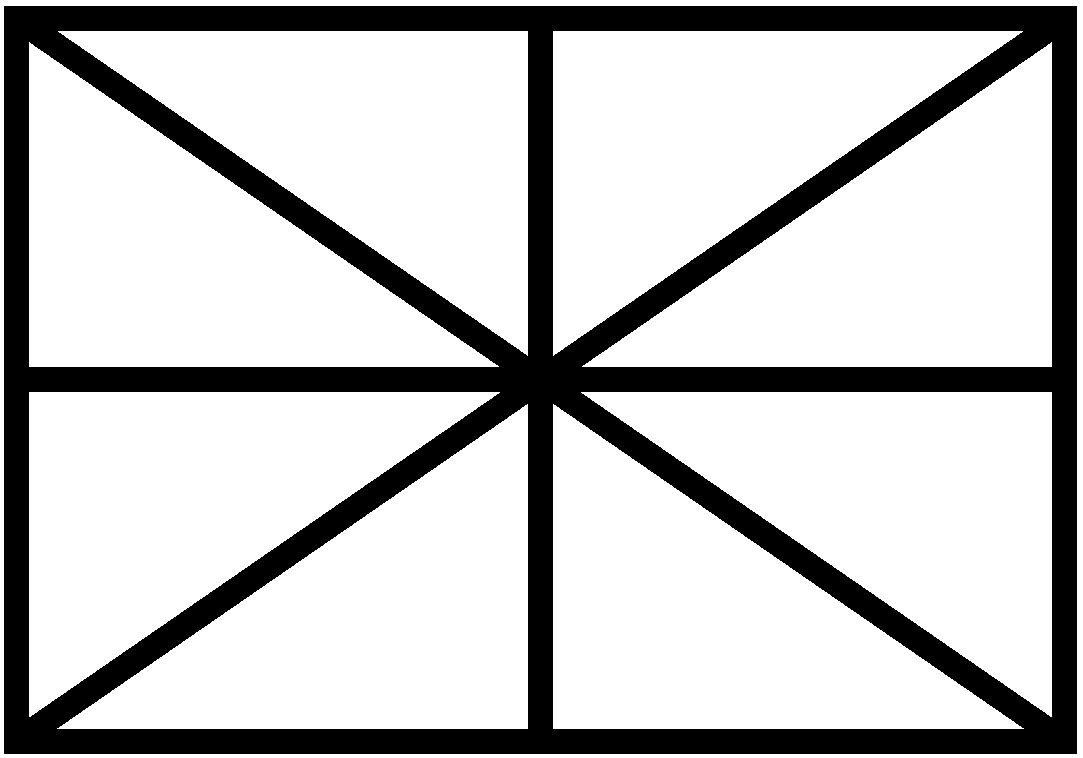
\includegraphics[width=\columnwidth]{figure.png}}}
 \caption{Figure captions should be placed below the figure.}
 \label{fig:example}
\end{figure}

\section{Equations}

Equations should be placed on separated lines and numbered.
The number should be on the right side, in parentheses.

\begin{equation}
E=mc^{2}
\end{equation}

\section{Citations}

All bibliographical references should be listed at the end,
inside a section named ``REFERENCES,'' numbered and in alphabetical order.
Also, all references listed should be cited in the text.
When referring to a document, type the numbering square brackets. \cite{Baeza-Yates1999}, \cite{Costa2008,Gouyon2011}

% \begin{thebibliography}{citations}

% \bibitem {Author:00}
% E. Author:
% ``The Title of the Conference Paper,''
% {\it Proceedings of the International Symposium
% on Music Information Retrieval}, pp.~000--111, 2000.

% \bibitem{Someone:10}
% A. Someone, B. Someone, and C. Someone:
% ``The Title of the Journal Paper,''
% {\it Journal of New Music Research},
% Vol.~A, No.~B, pp.~111--222, 2010.

% \bibitem{Someone:04} X. Someone and Y. Someone: {\it Title of the Book},
%     Editorial Acme, Porto, 2012.

% \end{thebibliography}

\bibliography{../report/bib/myrefs}
\bibliographystyle{unstrnat}

\end{document}
